\documentclass[../nirs.tex]{subfiles}
\usepackage{rotating}

\begin{document}
\section{Выявление основных понятий и процессов, их свойств и закономерностей.
Построение ER-диаграммы предметной области}

\subsection{Основные понятия}
Техническое обслуживание (ТО) -- это комплекс организационно-технических мероприятий
и работ, производимых на объекте и направленных на поддержание в рабочем или
исправном состоянии оборудования технических систем в процессе их использования
по назначению, с целью повышения надежности и эффективности их работы
[\ref{ref:техническое-обслуживание}].

Текущий ремонт (ТР) -- устранение мелких неисправностей и отказов автомобиля.
Способствует выполнению установленных норм пробега автомобиля до капитального
ремонта. Текущий ремонт заключается в проведении разборочно-сборочных,
слесарных, сварочных и других работ, а также в замене деталей в автомобиле
(прицепе, полуприцепе) [\ref{ref:му-ремонт-и-техническое-обслуживание}].

\subsection{Основные процессы}
Разрабатываемая информационная система должна обеспечивать выполнение следующих
бизнес-процессов:
\begin{itemize}
	\item обеспечивать просмотр и редактирование информации о конкретном
		автомобиле;
	\item обеспечивать просмотр и редактирование информации о текущем статусе
		работ;
	\item обеспечивать просмотр и редактирование информации о сотрудниках;
	\item обеспечивать просмотр и редактирование информации о доступных на
		складе ресурсах;
	\item прогнозировать дату окончания выполнения работ;
	\item составлять график прохождения технического обслуживания и ремонта
		техникой.
\end{itemize}

\subsection{Построение ER-диаграммы предметной области}
В автоматизированных информационных системах отражение предметной области
представлено моделями данных нескольких уровней:
\begin{enumerate}
	\item Инфологический.
	\item Даталогический.
	\item Физический.
\end{enumerate}

На каждом уровне проводится структуризация информации таким образом, чтобы на
третьем уровне информация могла быть представлена в виде структур данных,
реализуемых в памяти ЭВМ.

В результате исследования предметной области строится ее инфологическая модель,
которая описывается в терминах классов объектов и их взаимодействий. В
инфологической модели определяется какая информация о предметной области будет
хранится и обрабатываться в компьютере. Информация представляется вне
зависимости от того, что представляют собой данные и какие технические средства
будут использовании в дальнейшем для ее хранения и обработки. Цель инфологического
проектирования заключается в представлении семантики (смысла) предметной
области. Для описания предметной области наиболее часто используется модель
\textquote{сущность–связь}, которую сокращенно называют ER–моделью от
английского названия \textquote{Entity – Relationship} (\textquote{Сущность –
связь}). ER–диаграмма модели имеет лексикографическую структуру и включает в
себя текст и элементы графики [\ref{ref:er-диаграммы}].

При проектировании структуры предметной области определяют сущности (объекты,
явления), которые должны найти свое отражение в будущей системе.
Цель инфологического этапа проектирования состоит в получении семантических
(концептуальных) моделей, отражающих предметную область и информационные
потребности пользователей.

Классовая диаграмма разрабатываемой системы представлена на рисунке
\ref{fig:2_1_3_er_diagram}.

\begin{figure}[hp!]
	\centering
	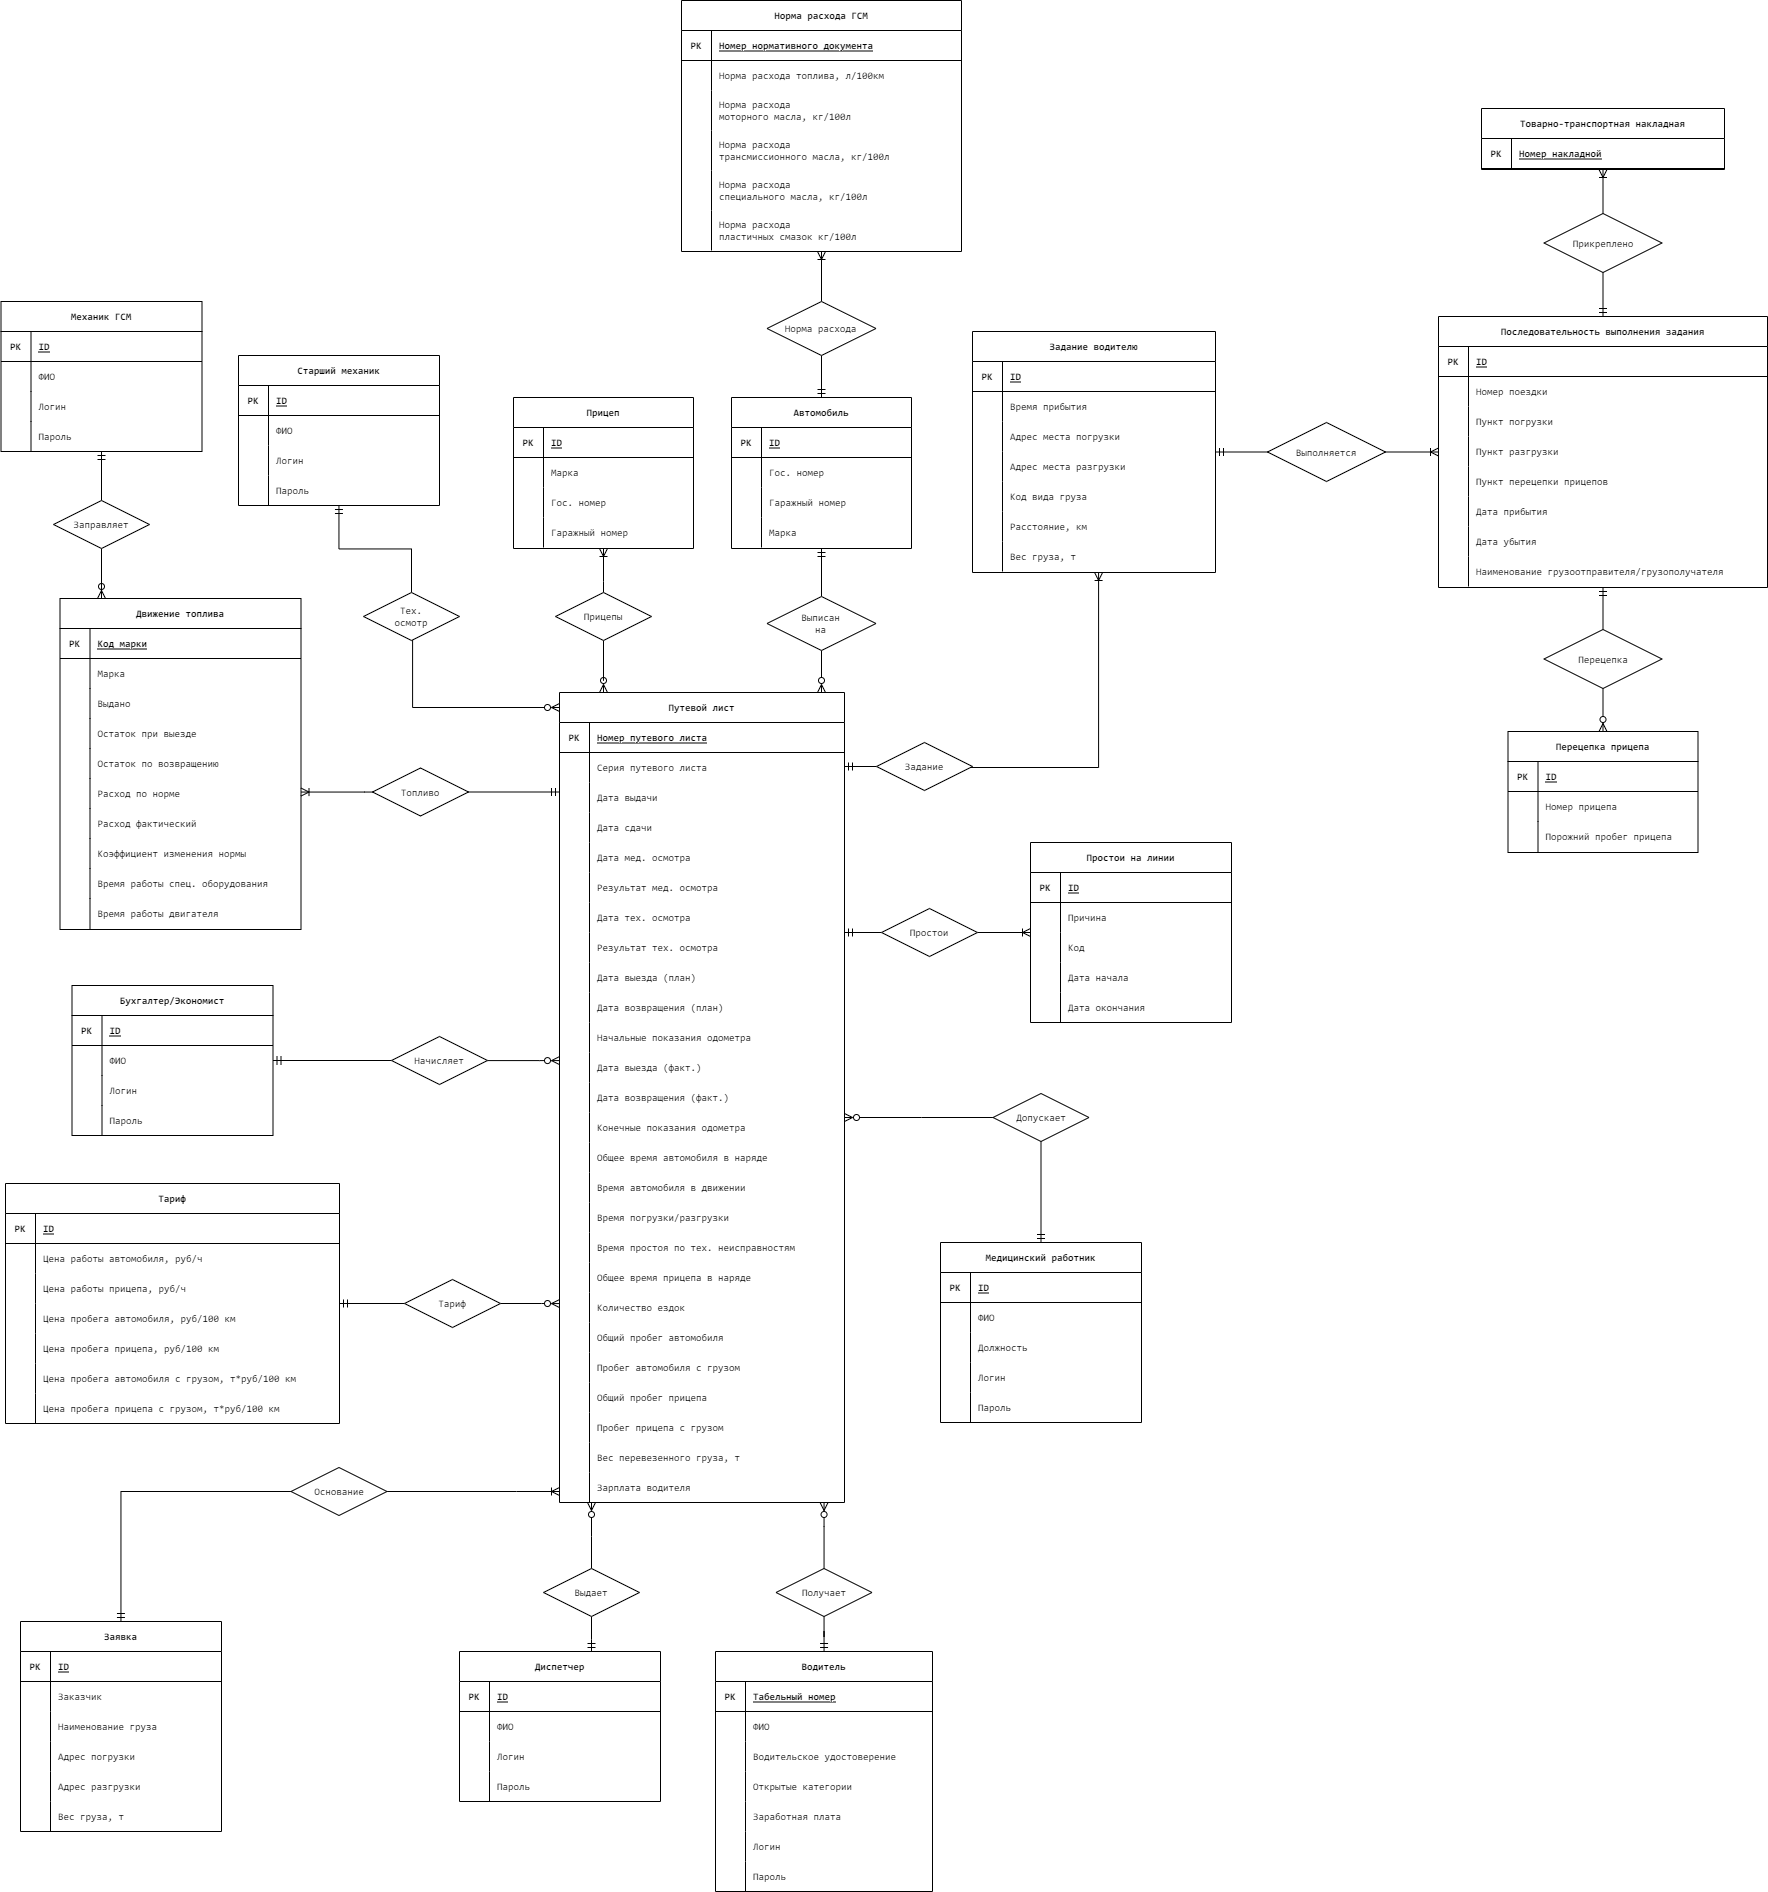
\includegraphics[keepaspectratio,width=\textwidth]{./images/2_1_3_er-diagram.png}
	\caption{ER-диаграмма системы}
	\label{fig:2_1_3_er_diagram}
\end{figure}

\pagebreak

Центральной сущностью выступает \textquote{Путевой лист}, являющийся
электронным аналогом путевого листа, заполняющегося на бумажном носителе.
Путевые листы формируются на основе заявок от заказчиков.

Диспетчер принимает заявку от заказчика и, посредством заранее созданных
экономистом тарифов на оплату услуг компании, рассчитывает ее стоимость. Вслед
за этим он выписывает путевые листы на каждую единицу техники, требующуюся для
выполнения данной заявки и формирует задание водителю, в котором указываются:
\begin{itemize}
	\item время подачи техники на место погрузки;
	\item адрес места погрузки;
	\item адрес места разгрузки;
	\item код вида груза;
	\item вес груза;
	\item расстояние между пунктами погрузки и разгрузки.
\end{itemize}

Во время выполнения задания, водитель заполняет последовательность выполнения
задания. В ней указывается порядковый номер поездки; адреса пункта погрузки,
пункта разгрузки, и, при необходимости, пункта перецепки прицепов; даты убытия с
места погрузки и прибытия на пункт разгрузки; наименование грузоотправителя
и/или грузополучателя. Для подтверждения факта транспортировки груза в путевом
листе прикладываются номера товарно-транспортных накладных на перевозимые грузы.

Старший механик проводит технический осмотр техники, с целью выявления ее
технического состояния. Заключение о техническом состоянии техники
вносится в путевой лист. При необходимости проведения технических работ
автомобиль отправляют в сервис. Перед выпуском автомобиля из гаража, а также по
его возвращении со смены старший механик проверяет и фиксирует показания
одометра в путевом листе.

Медицинский работник проводит медицинский осмотр водителя, назначенного на
выполнение задания. Результат осмотра фиксируется в путевом листе.

Механик ГСМ проверяет уровень топлива в автомобиле перед его выездом из гаража и
по возвращению со смены. В случае необходимости, заправляет автомобиль.
Количество залитого топлива фиксируется в путевом листе.

По закрытию путевого листа бухгалтер/экономист рассчитывает заработную плату
водителя, списывает израсходованные водителем ГСМ.

\end{document}
